% ********** Rozdział 2 **********
\chapter{Opis struktury projektu}
\section{Wstęp}
Projekt „Zarządzanie Pojazdami” został zrealizowany jako aplikacja desktopowa stworzona w języku C\# przy użyciu platformy .NET 8. Struktura projektu została zaprojektowana w sposób modułowy, co pozwala na łatwą rozbudowę i utrzymanie systemu. W niniejszym rozdziale omówiono techniczne aspekty projektu, jego architekturę, narzędzia użyte podczas implementacji oraz szczegóły dotyczące zarządzania danymi i integracji z bazą danych SQL.

\section{Język programowania, narzędzia i wymagania sprzętowe}
\subsection*{Język programowania}  
Aplikacja została napisana w języku C\# z wykorzystaniem platformy .NET 8, co zapewnia wysoką wydajność oraz możliwość uruchamiania na systemach Windows i Linux. C\# jako język obiektowy ułatwia zarządzanie pamięcią i wspiera nowoczesne techniki programowania, takie jak programowanie asynchroniczne. Zastosowanie .NET 8 pozwala na optymalizację wydajności, integrację z bazami danych SQL oraz łatwą rozbudowę aplikacji w przyszłości.% ********** Koniec rozdziału **********
\subsection*{Narzędzia użyte podczas tworzenia projektu:} 
\begin{itemize}
    \item Visual Studio – środowisko programistyczne wykorzystywane do implementacji i debugowania kodu.
    \item SQL Server Management Studio (SSMS) – narzędzie do zarządzania bazą danych SQL.
    \item Microsoft SQL Server – baza danych wykorzystywana do przechowywania informacji o pojazdach.
\end{itemize}
\section{Minimalne wymagania sprzętowe}
\begin{itemize}
    \item Procesor: Dwurdzeniowy, 1.8 GHz lub nowszy.
    \item Pamięć RAM: 2 GB (zalecane 4 GB dla lepszej wydajności).
    \item Dysk twardy: 250 MB wolnego miejsca na pliki aplikacji i bazę danych.
    \item System operacyjny: Windows 10/11 lub Linux z obsługą .NET 8.
\end{itemize}
\section{Zarządzanie danymi i integracja z bazą danych SQL}
System zarządza danymi pojazdów poprzez operacje na plikach TXT oraz bazie danych SQL.
\begin{itemize}
    \item Pliki TXT służą do lokalnego przechowywania danych i eksportu/importu informacji.
    \item Baza SQL zapewnia centralne przechowywanie pojazdów, umożliwiając ich szybkie przeszukiwanie i manipulację.
\end{itemize}
W aplikacji zastosowano Microsoft.Data.SqlClient do komunikacji z bazą danych SQL, co zapewnia efektywne wykonywanie operacji CRUD (Create, Read, Update, Delete).
Dodatkowo, aplikacja umożliwia importowanie danych z plików TXT do bazy SQL. Proces ten obejmuje:
\begin{itemize}
\item Odczytanie danych z plików tekstowych.
\item Parsowanie i weryfikację poprawności rekordów.
\item Wstawienie unikalnych rekordów do bazy SQL, aby uniknąć duplikacji.
\item Obsługę błędów i logowanie wyników importu.
\end{itemize}
\section{Struktura tabel SQL}
Dame są przechowywane w bazie danych, gdzie każda encja posiada swoją tabelę.
\begin{itemize}
\item Pojazdy
\begin{itemize}
\item ID - Klucz główny
\item Typ - Typ pojazdu (np. Samochód, Motocykl, Autobus)
\item Marka - Marka pojazdu
\item Model - Model pojazdu
\item RokProdukcji - Rok produkcji pojazdu
\item NumerRejestracyjny - Numer rejestracyjny pojazdu
\item DataDodania - Data dodania pojazdu do bazy
 \end{itemize}
\end{itemize}

\begin{itemize}
    \item Autobusy
    \begin{itemize}
        \item ID
        \item LiczbaMiejsc - Liczba miejsc w autobusie
        \item Dlugosc - Długość autobusu
    \end{itemize}
\end{itemize}
\begin{itemize}
    \item Ciezarowki
    \begin{itemize}
        \item ID
        \item Ladownosc - Ładowność ciężarówki
        \item Dlugosc - Długość ciężarówki
    \end{itemize}
\end{itemize}
\begin{itemize}
    \item Dostawczaki
    \begin{itemize}
        \item ID
        \item Ladownosc - Ładowność dostawczaka
    \end{itemize}
\end{itemize}
\begin{itemize}
    \item Motocykle
    \begin{itemize}
        \item ID
        \item Pojemnosc - Pojemność silnika motocykla
    \end{itemize}
\end{itemize}
\begin{itemize}
    \item SamochodyOsobowe
    \begin{itemize}
        \item ID
        \item LiczbaMiejsc - Liczba miejsc w samochodzie osobowym
    \end{itemize}
\end{itemize}
\begin{itemize}
    \item SamochodyElektryczne
    \begin{itemize}
        \item ID
        \item LiczbaMiejsc - Liczba miejsc w samochodzie elektrycznym
        \item PojemnoscBaterii - Pojemność baterii w kWh
        \item Zasieg - Zasięg pojazdu w km  
    \end{itemize}
\end{itemize}


\section{Struktura klas i hierarchia obiektów}
\subsection*{Interfejsy}
\begin{itemize}
    \item IPojazd – definiuje podstawowe operacje dla pojazdów.
    \item IBazaDanych – określa metody obsługi bazy danych.
\end{itemize}
\subsection*{Klasy abstrakcyjne}
\begin{itemize}
    \item Pojazd – klasa bazowa dla różnych typów pojazdów, zawierająca wspólne atrybuty i metody.
    \item BazaDanychBase – klasa abstrakcyjna dla różnych implementacji baz danych.
\end{itemize}
\subsection*{Klasy konkretne}
\begin{itemize}
    \item Autobus, Ciezarowka, Motocykl, SamochodOsobowy, SamochodElektryczny, Dostawczak – klasy dziedziczące po Pojazd, zawierające specyficzne właściwości.
    \item BazaDanych – implementacja operacji na danych w plikach TXT.
    \item BazaDanychSQL – obsługa bazy SQL.
    \item BazaDanychHybrydowa – klasa łącząca obsługę plików TXT i bazy SQL.
\end{itemize}
\subsection*{Diagram klas}
\clearpage
\begin{figure}[h] 
    \centering
    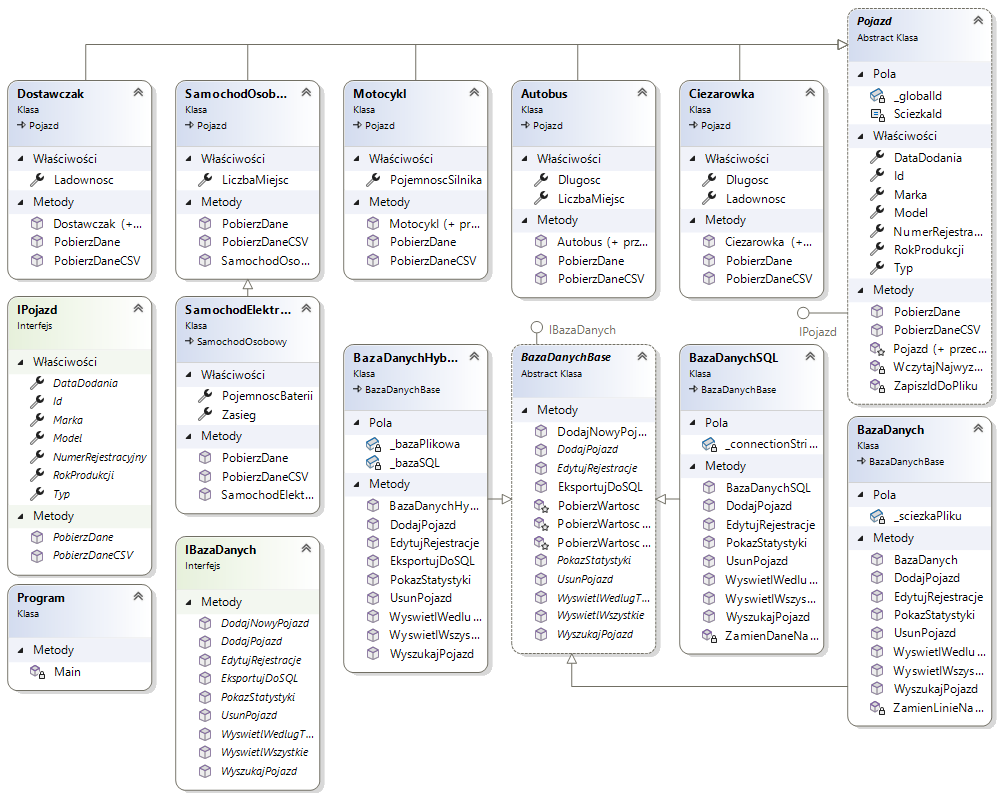
\includegraphics[width=1\textwidth]{Diagram klas.png}
    \caption{Diagram klas}
    \label{fig:moj_obrazek}
\end{figure}
\section{Opis najważniejszych metod}
\begin{itemize}
    \item DodajPojazd(IPojazd pojazd) – dodaje pojazd do bazy danych.
    \item UsunPojazd(string rejestracja) – usuwa pojazd na podstawie numeru rejestracyjnego.
    \item EdytujRejestracje(string staraRejestracja, string nowaRejestracja) – zmienia numer rejestracyjny pojazdu.
    \item WyszukajPojazd(string rejestracja) – wyszukuje pojazd po numerze rejestracyjnym.
    \item WyswietlWszystkie() – zwraca listę wszystkich pojazdów.
    \item WyswietlWedlugTypu(string typ) – zwraca listę pojazdów danego typu.
    \item PokazStatystyki() – generuje statystyki na podstawie danych.
    \item EksportujDoSQL(IBazaDanych sqlBaza) – eksportuje dane z plików TXT do bazy SQL.
\end{itemize}